\documentclass[tikz,border=2pt]{standalone}
\renewcommand{\familydefault}{\sfdefault}
\usetikzlibrary{arrows.meta,calc,positioning}
\tikzset{every picture/.style={line width=1pt, >=Stealth},
         hl/.style={fill=black, fill opacity=0.12, text opacity=1}}
\begin{document}
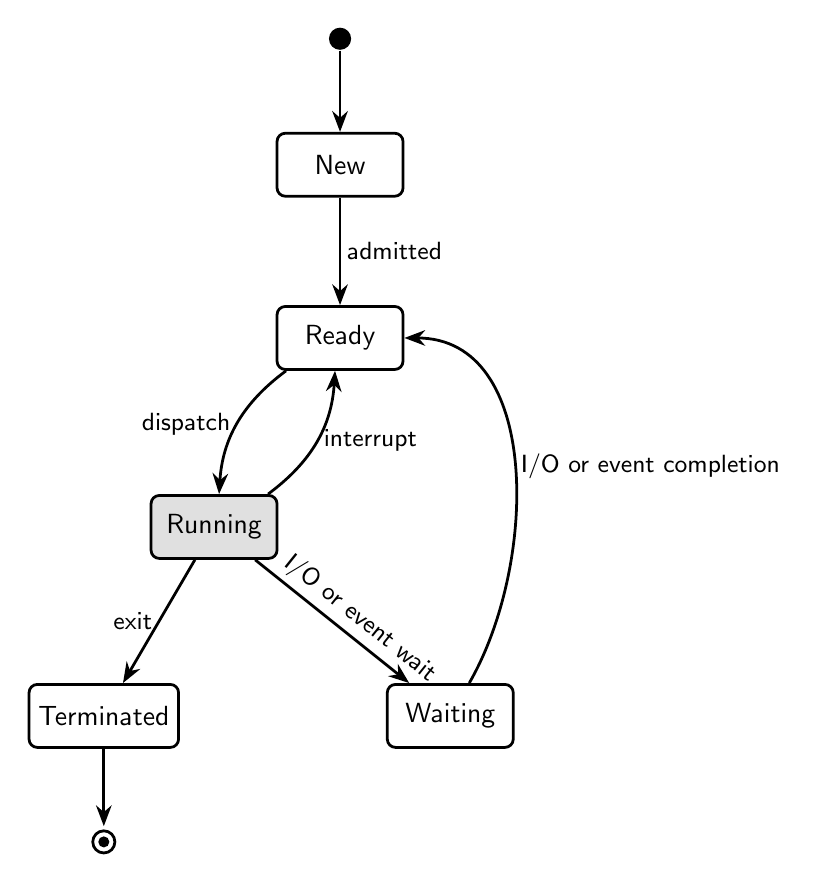
\begin{tikzpicture}[state/.style={draw, rounded corners=3pt, minimum height=0.8cm, minimum width=1.6cm},
    tag/.style={font=\small, inner sep=2pt}]
  \fill (3, 1.6) circle (4pt);
  \node[state] (new) at (3, 0) {New};
  \node[state] (ready) at (3, -2.2) {Ready};
  \node[state, hl] (run) at (1.4, -4.6) {Running};
  \node[state] (term) at (0, -7) {Terminated};
  \node[state] (wait) at (4.4, -7) {Waiting};
  \draw[->] (3, 1.45) -- (new);
  \draw[->] (new) -- node[tag, right] {admitted} (ready);
  \draw[->] (ready) to[bend right=25] node[tag, left] {dispatch} (run);
  \draw[->] (run) to[bend right=25] node[tag, right] {interrupt} (ready);
  \draw[->] (run) -- node[tag, left] {exit} (term);
  \draw[->] (run) -- node[tag, sloped, above, pos=0.6] {I/O or event wait} (wait);
  \draw[->] (wait) to[out=60, in=0] node[tag, right] {I/O or event completion} (ready);
  \draw[->] (term) -- (0, -8.4);
  \draw (0, -8.6) circle (4pt);
  \fill (0, -8.6) circle (2pt);
\end{tikzpicture}
\end{document}
